\begin{defn}[Graphs]\index{graph}\index{edge set}\index{vertex set}\index{graph!degree}\index{graph!total degree}
    A \emph{graph} consists of two finite sets: a nonempty \emph{set of vertices} and a \emph{set of edges}, where each edge is associated with a set consisting of either one or two vertices called its endpoints. The correspondence from edges to endpoints is called the edge-endpoint function.
\end{defn}
\begin{exposition} Here is some basic terminology:
\begin{sides}[righthand width=0.48\linewidth]
    \begin{figure}[H]
        \centering
        %\inputtikz{label_graph}
        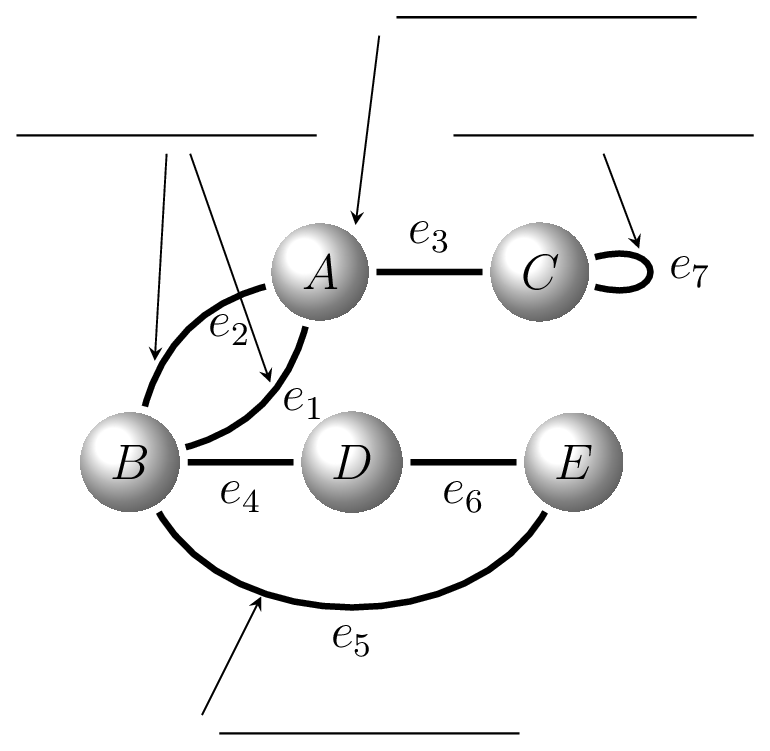
\includegraphics[scale=0.24,alt={}]{images/created/label_graph.png}
        \caption{Sample Graph}
        \label{fig:sample_graph}
    \end{figure}
\tcblower
        Vertex Set = {\Large\(\{\phantom{A,B,C,D,E}\}\)}\vspace{\baselineskip}\newline
        Edge Set = {\Large\(\{\phantom{e_1,e_2,e_3,e_4,e_5,e_6,e_7}\}\)}\vspace{\baselineskip}\newline
        Degrees:
        \begin{itemize}
            \item \(deg(A)=\)
            \item \(deg(B)=\)
            \item \(deg(C)=\)
            \item \(deg(D)=\)
            \item \(deg(E)=\)
            \item \(Total\ Degree=\)
        \end{itemize}
\end{sides}
\end{exposition}

\begin{exposition}\index{graph!complete}\index{graph!directed}\index{graph!digraph}\index{graph!bipartite}\index{graph!complete bipartite}\index{graph!tree}\index{graph!binary tree}
Below is a sampling of common types of graphs.
\begin{sides}
Complete Graph:
\begin{center}
    %\inputtikz{graph_complete}
    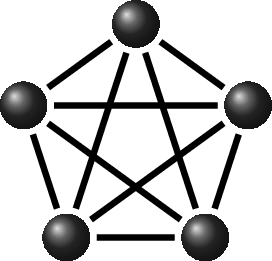
\includegraphics[scale=0.24,alt={}]{images/created/graph_complete.png}
\end{center}

Directed Graph (Digraph):
\begin{center}
    %\inputtikz{graph_directed}
    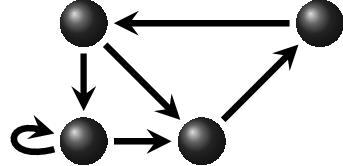
\includegraphics[scale=0.24,alt={}]{images/created/graph_directed.png}
\end{center}

Bipartite Graph:
\begin{center}
    %\inputtikz{graph_bipartite}
    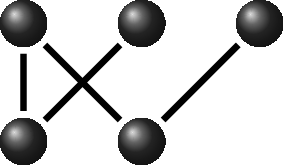
\includegraphics[scale=0.24,alt={}]{images/created/graph_bipartite.png}
\end{center}

\tcblower

Complete Bipartite Graph:
\begin{center}
    %\inputtikz{graph_bicomplete}
    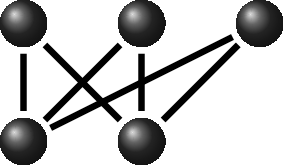
\includegraphics[scale=0.24,alt={}]{images/created/graph_bicomplete.png}
\end{center}

Tree:
\begin{center}
    %\inputtikz{graph_tree}
    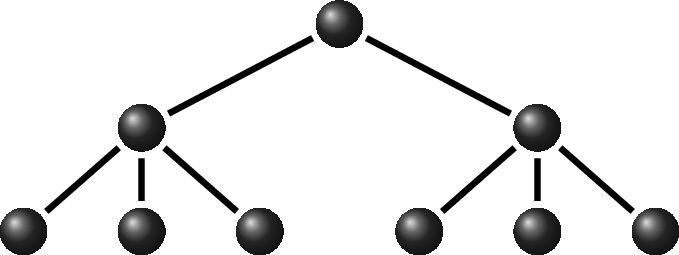
\includegraphics[scale=0.24,alt={}]{images/created/graph_tree.png}
\end{center}

Binary Tree:
\begin{center}
    %\inputtikz{graph_bitree}
    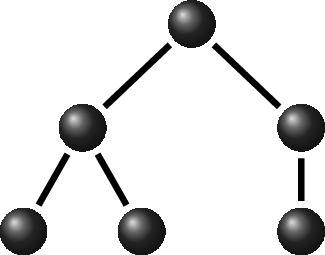
\includegraphics[scale=0.24,alt={}]{images/created/graph_bitree.png}
\end{center}
    
\end{sides}

\end{exposition}

\begin{thm}[Handshake Theorem]\index{handshake theorem}\index{total degree}{\index{graph!total degree}}
    If \(G\) is any graph, then the sum of the degrees of all the vertices of \(G\), the \emph{total degree}, equals twice the number of edges in \(G\).  Specifically, if\newline \(V=\{v_1,v_2,\ldots,v_n\}\) is the vertex set of \(G\) and \(E=\{e_1,e_2,\ldots,e_k\}\) is the edge set then
    \[total\ degree\ of\ G=\sum_{v_i\in V}deg(v_i)=2|E|=2k.\]
\end{thm}

\begin{cor}[Immediate Consequences]
    Let \(G\) be a graph with vertex set \(V\) and edge set \(E\), then
    \begin{enumerate}
        \item the total degree of \(G\) is even, and
        \item the number of vertices of odd degree is even.
    \end{enumerate}
\end{cor}

\begin{thm}
    If \(G\) is a \emph{complete graph} with \(n\) vertices, then \(G\) has \(_nC_k\) edges.
% \begin{center}
%     \begin{tikzpicture}
%         \graph[nodes={SolidVertex,empty nodes},edges={edges}] {subgraph K_n [n=5,clockwise]};
%     \end{tikzpicture}
% \end{center}
\end{thm}

\begin{thm}
    If \(G\) is a \emph{complete bipartite graph} with \(n\) vertices in one set and \(m\) in the other, then \(G\) has \(n\times m\) edges.
% \begin{center}
%     \begin{tikzpicture}
%         \graph[branch right,grow down,nodes={SolidVertex,empty nodes},edges={edges}]{subgraph K_nm [n=3,m=2]};
%     \end{tikzpicture}
% \end{center}
\end{thm}

\begin{defn}[Simple Graph]\index{simple graph} \index{graph!simple} \index{multigraph} \index{graph!multigraph}
    A \emph{simple graph} is a graph with no loops and no parallel edges.
    Note that, in some settings simple graphs are just called graphs, and graphs with loops or parallel edges are called \emph{multigraphs}.
\end{defn}

% \clearpage

\begin{practiceprob}
Find the vertex set, edge set, and degree for each vertex.  Is this a particular type of graph?

%\inputtikz{graph_practice}
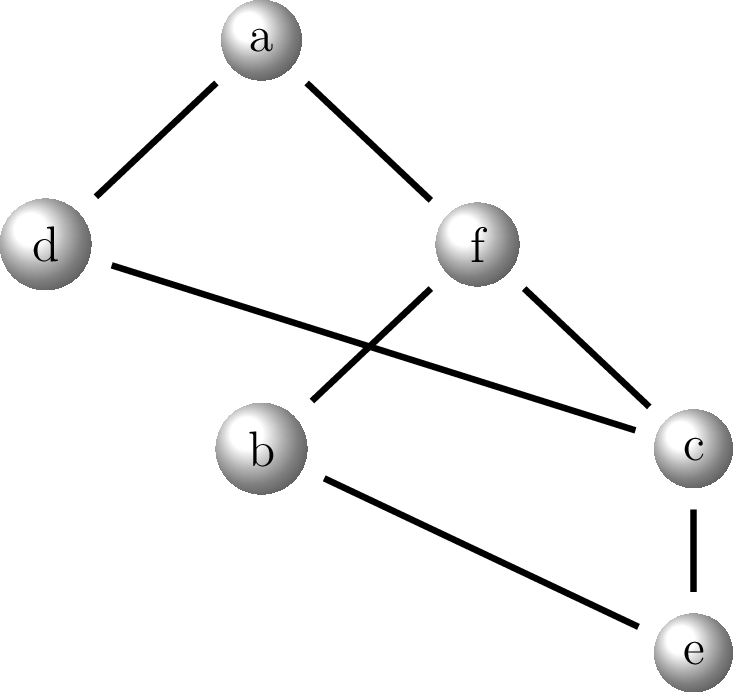
\includegraphics[scale=0.24,alt={}]{images/created/graph_practice.png}


\end{practiceprob}

\begin{practiceprob}
Construct a graph from the given information.\vspace{\baselineskip}

    \begin{tabular}{|c|c|}\hline
         Edges & End Points \tabularnewline\hline
         \(e_1\) & \(\{v_1,v_2\}\) \tabularnewline\hline
         \(e_2\) & \(\{v_1,v_2\}\) \tabularnewline\hline
         \(e_3\) & \(\{v_1,v_3\}\) \tabularnewline\hline
         \(e_4\) & \(\{v_2,v_3\}\) \tabularnewline\hline
         \(e_5\) & \(\{v_3,v_3\}\) \tabularnewline\hline
    \end{tabular}\vspace{5\baselineskip}

\end{practiceprob}

